% Generated from current Astra diagram sources.
\documentclass[border=12pt]{standalone}
\def\pgfsysdriver{pgfsys-dvisvgm.def}
\usepackage[dvisvgm]{xcolor}
\usepackage{xeCJK}
\setCJKmainfont{HaranoAjiGothic-Regular.otf}[BoldFont=HaranoAjiGothic-Bold.otf]
\setCJKsansfont{HaranoAjiGothic-Regular.otf}[BoldFont=HaranoAjiGothic-Bold.otf]
\usepackage{amsmath,amssymb,tikz,lmodern}
\usetikzlibrary{arrows.meta,positioning,calc,patterns}
\renewcommand{\familydefault}{\sfdefault}
\definecolor{ink}{HTML}{25322F}
\definecolor{green}{HTML}{246657}
\definecolor{tint}{HTML}{EEF4F0}
\definecolor{soft}{HTML}{C6D2CC}
\definecolor{muted}{HTML}{52615B}
\newif\ifJapanese
\newcommand{\Tx}[2]{\ifJapanese #1\else #2\fi}
\newcommand{\Head}[2]{{\color{green}\bfseries\Tx{#1}{#2}}\\[5pt]}
\newcommand{\refurl}[2]{\special{dvisvgm:raw <a xlink:href="#1" target="_blank" rel="noopener noreferrer">}{\setlength{\fboxsep}{0pt}\colorbox{white}{\color{green}\underline{\strut #2}}}\special{dvisvgm:raw </a>}}
\tikzset{box/.style={draw=soft,fill=white,rounded corners=2pt,text=ink,align=left,text width=14.2cm,inner sep=12pt,font=\fontsize{10.5}{14}\selectfont},result/.style={box,draw=green,fill=tint},reason/.style={text=muted,align=left,text width=12.5cm,font=\fontsize{9}{12}\selectfont,inner sep=0pt},edge/.style={-{Stealth[length=2.3mm]},line width=1pt,draw=green}}
\newcommand{\Flow}[3]{\draw[edge] ($(#1.south)+(-6.7,0)$)--($(#2.north)+(-6.7,0)$);\node[reason,anchor=west] at ($(#1.south)!.5!(#2.north)+(-6.2,0)$){#3};}
% Shared MIT-licensed repository typography; all catalogue-187 diagram content newly authored by Astra.

% Generated from citations.json; do not edit.
\newcommand{\Cite}[1]{\csname cite-#1\endcsname}
\expandafter\def\csname cite-rules\endcsname{\shortstack[l]{\refurl{https://github.com/openai/math/blob/1581d4cbdd69a0faf34b2089614fe2a814316a6a/preprints/Snaky-in-21-Maker-moves-September-25-2026/article.pdf}{§1; (1) · pp. 1–2}}}
\expandafter\def\csname cite-theorem\endcsname{\shortstack[l]{\refurl{https://github.com/openai/math/blob/1581d4cbdd69a0faf34b2089614fe2a814316a6a/preprints/Snaky-in-21-Maker-moves-September-25-2026/article.pdf}{Theorem 1 · p. 1}}}
\expandafter\def\csname cite-finite\endcsname{\shortstack[l]{\refurl{https://github.com/openai/math/blob/1581d4cbdd69a0faf34b2089614fe2a814316a6a/preprints/Snaky-in-21-Maker-moves-September-25-2026/article.pdf}{Corollary 6 · p. 8}}}
\expandafter\def\csname cite-condition\endcsname{\shortstack[l]{\refurl{https://github.com/openai/math/blob/1581d4cbdd69a0faf34b2089614fe2a814316a6a/preprints/Snaky-in-21-Maker-moves-September-25-2026/article.pdf}{Definition 2; §2 · p. 3}}}
\expandafter\def\csname cite-bases\endcsname{\shortstack[l]{\refurl{https://github.com/openai/math/blob/1581d4cbdd69a0faf34b2089614fe2a814316a6a/preprints/Snaky-in-21-Maker-moves-September-25-2026/article.pdf}{Lemma 4 · p. 4}}}
\expandafter\def\csname cite-certificate\endcsname{\shortstack[l]{\refurl{https://github.com/openai/math/blob/1581d4cbdd69a0faf34b2089614fe2a814316a6a/preprints/Snaky-in-21-Maker-moves-September-25-2026/article.pdf}{Proposition 5; (7) · pp. 5–6}}}
\expandafter\def\csname cite-policy\endcsname{\shortstack[l]{\refurl{https://github.com/openai/math/blob/1581d4cbdd69a0faf34b2089614fe2a814316a6a/preprints/Snaky-in-21-Maker-moves-September-25-2026/article.pdf}{§4 · pp. 7–8}}}
\expandafter\def\csname cite-combine\endcsname{\shortstack[l]{\refurl{https://github.com/openai/math/blob/1581d4cbdd69a0faf34b2089614fe2a814316a6a/preprints/Snaky-in-21-Maker-moves-September-25-2026/article.pdf}{Lemma 3; (2)–(3) · pp. 3–4}}}
\expandafter\def\csname cite-elementary\endcsname{\shortstack[l]{\refurl{https://github.com/openai/math/blob/1581d4cbdd69a0faf34b2089614fe2a814316a6a/preprints/Snaky-in-21-Maker-moves-September-25-2026/article.pdf}{§3.2; (6); Figure 2 · pp. 5–6}}}
\expandafter\def\csname cite-encoding\endcsname{\shortstack[l]{\refurl{https://github.com/openai/math/blob/1581d4cbdd69a0faf34b2089614fe2a814316a6a/preprints/Snaky-in-21-Maker-moves-September-25-2026/article.pdf}{§3.1 · pp. 4–5}}}
\expandafter\def\csname cite-intersection\endcsname{\shortstack[l]{\refurl{https://github.com/openai/math/blob/1581d4cbdd69a0faf34b2089614fe2a814316a6a/preprints/Snaky-in-21-Maker-moves-September-25-2026/article.pdf}{§3.3; Table 1 · pp. 6–7}}}
\expandafter\def\csname cite-verification\endcsname{\shortstack[l]{\refurl{https://github.com/openai/math/blob/1581d4cbdd69a0faf34b2089614fe2a814316a6a/preprints/Snaky-in-21-Maker-moves-September-25-2026/article.pdf}{§6.1 · pp. 11–12}}}
\expandafter\def\csname cite-program\endcsname{\shortstack[l]{\refurl{https://github.com/openai/math/blob/1581d4cbdd69a0faf34b2089614fe2a814316a6a/preprints/Snaky-in-21-Maker-moves-September-25-2026/article.pdf}{Appendix G.2 · pp. 82–84}}}
\expandafter\def\csname cite-supplement\endcsname{\shortstack[l]{\refurl{https://github.com/openai/math/blob/1581d4cbdd69a0faf34b2089614fe2a814316a6a/preprints/Snaky-in-21-Maker-moves-September-25-2026/article.pdf}{Appendix G.1 · pp. 81–82}}}

\Japanesetrue
\begin{document}
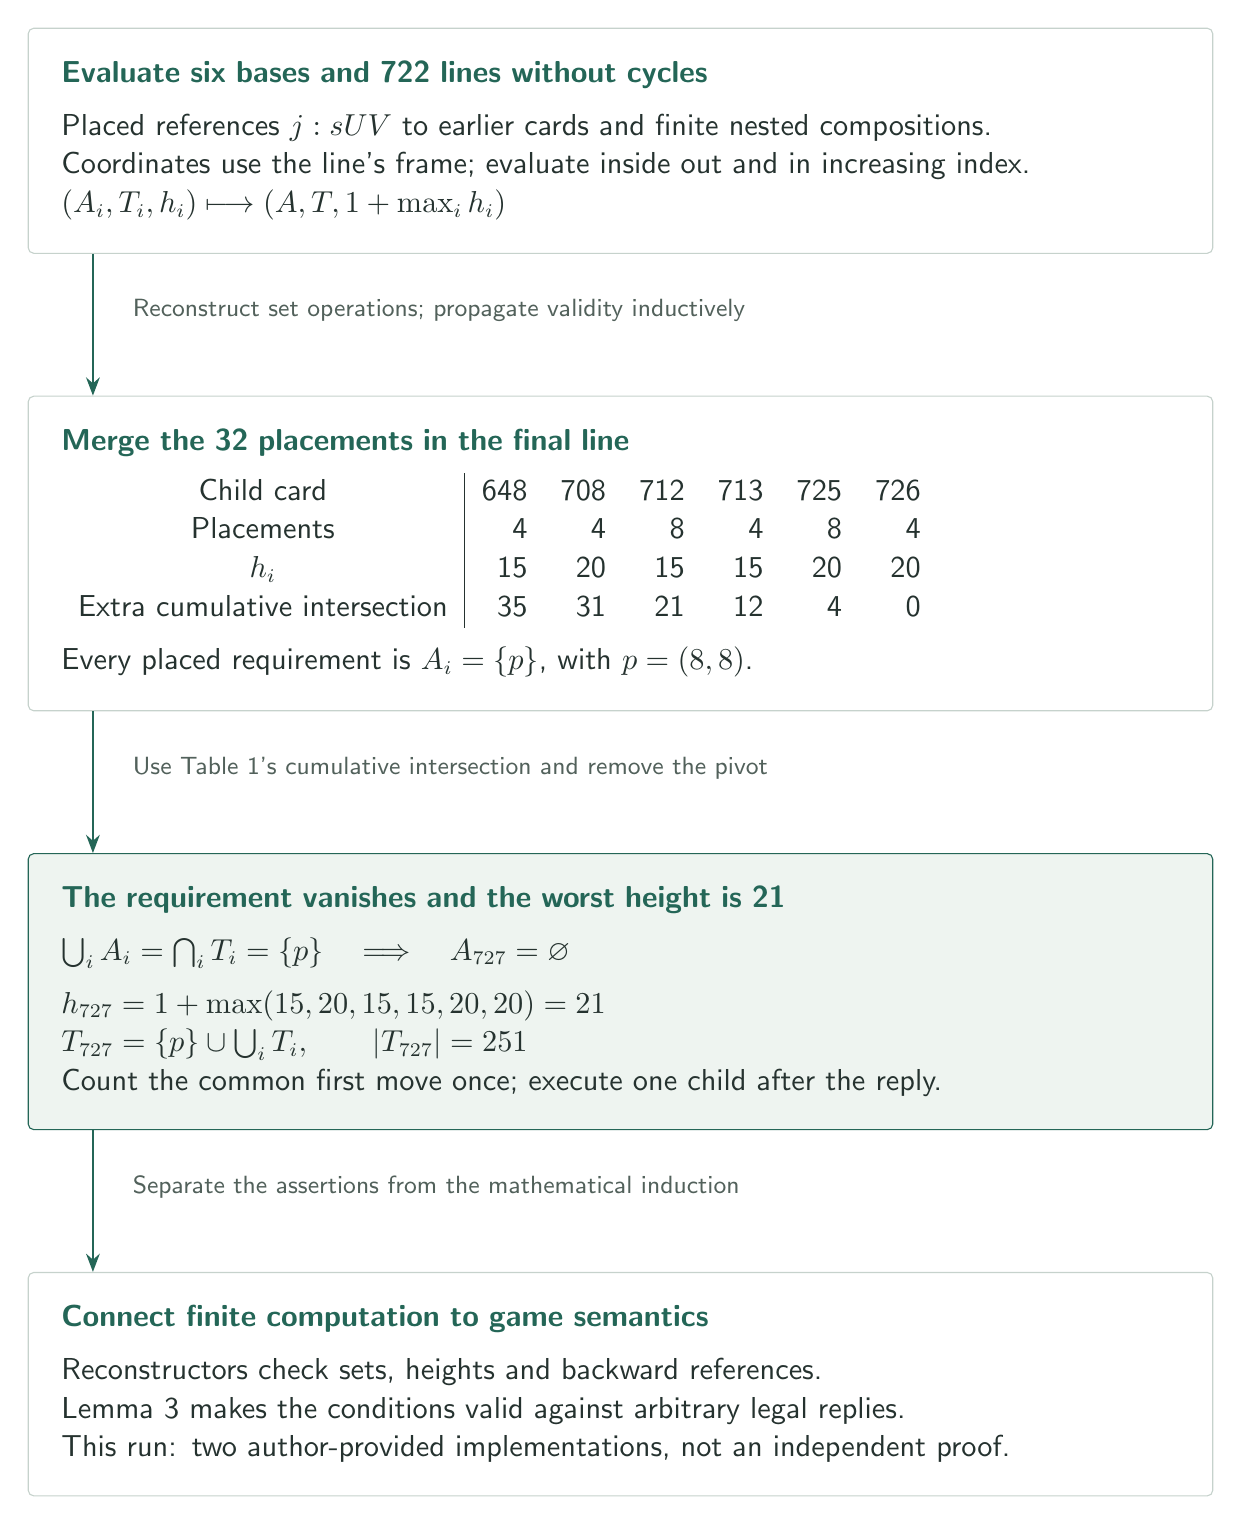
\begin{tikzpicture}
\node[box] (a) {\Head{六基底と722行を、循環なく評価する}{Evaluate six bases and 722 lines without cycles}
\Tx{既出cardの配置参照 $j:sUV$ と、有限な括弧内合成。}{Placed references $j:sUV$ to earlier cards and finite nested compositions.}\\
\Tx{座標は行の座標系。括弧は内側から、番号は小さい側から。}{Coordinates use the line's frame; evaluate inside out and in increasing index.}\\
$(A_i,T_i,h_i)\longmapsto(A,T,1+\max_i h_i)$};
\node[box,below=1.8cm of a] (b) {\Head{最終行の32配置へ合流する}{Merge the 32 placements in the final line}
\begin{tabular}{c|rrrrrr}
\Tx{子card}{Child card}&648&708&712&713&725&726\\
\Tx{配置数}{Placements}&4&4&8&4&8&4\\
$h_i$&15&20&15&15&20&20\\
\Tx{余分な累積交差}{Extra cumulative intersection}&35&31&21&12&4&0
\end{tabular}\\[6pt]
\Tx{すべての配置後の $A_i=\{p\}$、$p=(8,8)$。}{Every placed requirement is $A_i=\{p\}$, with $p=(8,8)$.}};
\Flow{a}{b}{\Tx{集合演算を再構成し、各条件の有効性を帰納的に伝える}{Reconstruct set operations; propagate validity inductively}\\\Cite{encoding}\quad\Cite{certificate}}
\node[result,below=1.8cm of b] (c) {\Head{要求が空になり、最悪の高さが21になる}{The requirement vanishes and the worst height is 21}
$\bigcup_i A_i=\bigcap_iT_i=\{p\}\quad\Longrightarrow\quad A_{727}=\varnothing$\\[5pt]
$h_{727}=1+\max(15,20,15,15,20,20)=21$\\
$T_{727}=\{p\}\cup\bigcup_i T_i,\qquad |T_{727}|=251$\\
\Tx{同じ初手を一度だけ数え、応手後に一つの子を実行する。}{Count the common first move once; execute one child after the reply.}};
\Flow{b}{c}{\Tx{Table 1の累積交差を使い、ピボットを要求から除く}{Use Table 1's cumulative intersection and remove the pivot}\\\Cite{intersection}\quad\Cite{combine}}
\node[box,below=1.8cm of c] (d) {\Head{有限計算とゲームの意味を接続する}{Connect finite computation to game semantics}
\Tx{再構成器：集合・高さ・後方参照を検査。}{Reconstructors check sets, heights and backward references.}\\
\Tx{Lemma 3：その条件が任意の合法応手に耐えることを保証。}{Lemma 3 makes the conditions valid against arbitrary legal replies.}\\
\Tx{今回：著者の二実装を再実行。独自の独立証明ではない。}{This run: two author-provided implementations, not an independent proof.}};
\Flow{c}{d}{\Tx{assertの対象と数学的帰納法の役割を区別する}{Separate the assertions from the mathematical induction}\\\Cite{verification}\quad\Cite{program}}

\end{tikzpicture}
\end{document}
